\documentclass[11pt,a4paper]{article}

\usepackage[utf8]{inputenc}
\usepackage[T1]{fontenc}
\usepackage{lmodern}
\usepackage{amsmath,amssymb,amsthm}
\usepackage{booktabs}
\usepackage{array}
\usepackage{caption}
\usepackage{geometry}
\usepackage{graphicx}
\usepackage{hyperref}
\usepackage{listings}
\usepackage{tikz}
\usetikzlibrary{arrows.meta,positioning,calc}
\usepackage{xcolor}
\usepackage{microtype}

\geometry{margin=1in}
\setlength{\emergencystretch}{3em}

\captionsetup[lstlisting]{singlelinecheck=false,justification=raggedright}

\hypersetup{
  colorlinks=true,
  linkcolor=blue!60!black,
  citecolor=green!50!black,
  urlcolor=blue!60!black
}

\lstdefinelanguage{Lean4}{
  morekeywords={def,theorem,lemma,abbrev,by,rfl,let,in,if,then,else,match,with,fun,true,false,set_option},
  sensitive=true,
  morecomment=[l]{--},
  morecomment=[s]{/-}{-/},
  morestring=[b]"
}

\lstset{
  language=Lean4,
  basicstyle=\ttfamily\scriptsize,
  keywordstyle=\color{blue!70!black}\bfseries,
  commentstyle=\color{gray!70!black}\itshape,
  stringstyle=\color{green!50!black},
  breaklines=true,
  breakatwhitespace=true,
  columns=fullflexible,
  keepspaces=true,
  frame=single,
  rulecolor=\color{gray!35},
  backgroundcolor=\color{gray!5},
  xleftmargin=0.4em,
  xrightmargin=0.4em,
  aboveskip=0.6em,
  belowskip=0.6em,
  literate={⟨}{{$\langle$}}1 {⟩}{{$\rangle$}}1 {×}{{$\times$}}1 {→}{{$\to$}}1 {↠}{{$\twoheadrightarrow$}}1 {∧}{{$\land$}}1 {·}{{$\cdot$}}1 {±}{{$\pm$}}1 {∈}{{$\in$}}1 {∘}{{$\circ$}}1 {∪}{{$\cup$}}1 {⊂}{{$\subset$}}1 {⊆}{{$\subseteq$}}1 {⊕}{{$\oplus$}}1 {⊗}{{$\otimes$}}1 {⋀}{{$\bigwedge$}}1 {≤}{{$\le$}}1 {≥}{{$\ge$}}1 {≠}{{$\neq$}}1 {∨}{{$\lor$}}1
}

\newtheorem{theorem}{Theorem}[section]
\newtheorem{proposition}[theorem]{Proposition}
\newtheorem{definition}[theorem]{Definition}
\newtheorem{remark}[theorem]{Remark}

\title{\textbf{Constructive Formalization of \texorpdfstring{$\operatorname{Spin}(8)$}{Spin(8)} Triality, \texorpdfstring{$W(D_4)$}{W(D4)} Chiral Orthogonality, and Mumford Spinor Representations in Lean~4}}

\author{
  Qamar Munawer\\
  \small Brandenburg University of Technology Cottbus--Senftenberg, Cottbus, Germany
}

\date{}

\begin{document}
\maketitle

\begin{abstract}
This paper presents a constructive, axiom-free formalization in Lean~4 of the finite-dimensional Lie-theoretic weight combinatorics, full $24$-root Weyl reflection group theory, order-$3$ outer triality automorphism, and root-operator linear algebra underlying Mumford's spinor Hodge classes on abelian varieties of $D_4$ type. It formalizes the discrete weight spaces, exterior-power chiral splittings, subalgebra Casimir Gram kernels, and exact group-character orthogonality of $\operatorname{Spin}(8)$ representations. With no external library imports, the Lean~4 kernel generates the $8$-dimensional vector and half-spinor weight spaces from first principles, proves commutative-associative lattice laws across $S^+_8 \cup S^-_8 \cup V_8$ with zero axioms, verifies Weyl reflection invariance across all $24$ roots of $\Phi(D_4)$ and order-$3$ outer triality $\tau : V_8 \to S^+_8 \to S^-_8 \to V_8$, counts the $32$ triality zero-sum triples, verifies the Hodge-star splitting of $\bigwedge^4 S^+_8$ into $35_+ \oplus 35_-$ and invertibility of the $6 \times 6$ Weyl-to-Weil transition matrix, certifies full rank $6$ for both $D_4$ and triality-conjugate $A_3$ Gram matrices versus rank $4$ (kernel $2$) on $A_1^3$ and $A_2$ subsystems, and evaluates exact character inner products over all $192$ elements of $W(D_4)$.
\end{abstract}

\section{Introduction and Mathematical Setting}

Abelian fourfolds of Mumford type~\cite{Mumford1969,Weil1977} provide the canonical examples of exceptional Hodge classes that are not generated by intersections of divisor classes. For a general abelian fourfold whose Mumford--Tate group is isogenous to $\operatorname{Spin}(8)$ (or a $\mathbb{Q}$-form of $D_4$), the first cohomology $H^1(A, \mathbb{Q})$ carries an $8$-dimensional spinor representation, and the middle cohomology $H^4(A, \mathbb{Q}) \cong \bigwedge^4 H^1(A, \mathbb{Q})$ decomposes under $\mathfrak{so}(8)$ into irreducible representations including the $35$-dimensional self-dual and anti-self-dual components $35_+ \oplus 35_-$. Weil's Hodge classes~\cite{Weil1977,vanGeemen1994,Zarhin1984} arise inside the $6$-dimensional Cartan zero-weight space $(\bigwedge^4 S^+_8)_0$, where triality relates the vector representation $V_8$ and the two half-spinor representations $S^+_8$ and $S^-_8$~\cite{Voisin2002}.

A systematic audit of \texttt{mathlib4} and existing Lean~4 formalizations shows zero prior implementations of $\operatorname{Spin}(8)$ triality, the full $24$-root $\Phi(D_4)$ Weyl system, the $192$-element Weyl group $W(D_4) \cong S_4 \ltimes (\mathbb{Z}/2\mathbb{Z})^3$, Hodge-star chiral splitting on $\bigwedge^4 S^+_8$, or Jordan--Wigner root-action Gram matrices. This paper presents a constructive, axiom-free formalization of these Lie-theoretic invariants in Lean~4.35.0 spanning \texttt{ShiodaFormalConjectures.lean}, \texttt{HodgeVerification.lean}, the triality module \texttt{MathlibPR\_Spin8Triality.lean}, and the full root-system module \texttt{Spin8LieAlgebraTriality.lean}.

\begin{remark}[Mathematical Scope]
  The formal theorems verified in Lean~4 establish finite-dimensional representation-theoretic identities, weight-space cardinalities, matrix invertibility, triality bijections, subalgebra Gram ranks, and Weyl character inner products for $\mathfrak{so}(8) = D_4$, providing the Lie-algebraic kernel for Mumford--Weil Hodge reductions.
\end{remark}

\subsection{Geometric Intuition: Triality Symmetry and Singlet Annihilation in Closed Spinor Systems}

The Lie algebra $\mathfrak{so}(8)$ of type $D_4$ occupies a unique position among all simple Lie algebras because its Dynkin diagram possesses an outer automorphism group $\operatorname{Out}(\mathfrak{so}(8)) \cong S_3$. An order-$3$ outer triality automorphism $\tau = H_{\mathrm{tri}} \circ r_3$ rotates the three peripheral simple roots $\alpha_1 \to \alpha_4 \to \alpha_3 \to \alpha_1$ around the fixed central root $\alpha_2$ while cyclically permuting the three $8$-dimensional fundamental representations $V_8 \to S^+_8 \to S^-_8 \to V_8$ as a strict closed weight system ($\tau^3 = \mathrm{id}$).

To isolate exceptional Hodge classes inside $H^4(A, \mathbb{Q}) \cong \bigwedge^4 S^+_8$, representation theory compresses the search to the $6$-dimensional Cartan zero-weight subspace $(\bigwedge^4 S^+_8)_0 = 3_+ \oplus 3_-$, where every $\mathfrak{so}(8)$-invariant Hodge class must reside. Stacking the Jordan--Wigner raising operators $E_\alpha$ across all roots $\alpha \in \Delta(D_4)$ or $\Phi(D_4)$ defines a finite Casimir / simple-root Gram operator whose kernel consists precisely of the trivial $\mathfrak{so}(8)$ singlets. Because this Gram matrix attains full rank $6$, no trivial $\mathfrak{so}(8)$ singlet survives on $(\bigwedge^4 S^+_8)_0$. Exceptional Weil Hodge classes emerge only when the ambient symmetry breaks to a proper Mumford--Tate subalgebra: restricting the same Gram operator to the peripheral $A_1^3 = \{\alpha_1, \alpha_3, \alpha_4\}$ or connected $A_2$ root subsystems drops the rank from $6$ to $4$, leaving behind an exact $2$-dimensional invariant Weil Hodge kernel inside the $6$-dimensional zero-weight space.

\section{Constructive Generation of \texorpdfstring{$\operatorname{Spin}(8)$}{Spin(8)} Weight Spaces and Triality Zero-Sum Triples}

Using scaled integer coordinates ($2\times$ the standard half-integer lattice $\frac{1}{2}(\pm 1, \pm 1, \pm 1, \pm 1)$), the $16$ sign tuples in $\{\pm 1\}^4$ are generated algorithmically by \texttt{allSign4Tuples}. Filtering by sign product $+1$ yields the $8$ weights of the even half-spinor representation $S^+_8$ (\texttt{so8Weights}), while sign product $-1$ yields the $8$ weights of the odd half-spinor representation $S^-_8$ (\texttt{so8OddSpinorWeights}). The $8$ weights of the vector representation $V_8$ (\texttt{so8VectorWeights}) are the coordinate vectors $\pm 2 e_i$ for $0 \le i \le 3$.

The even Clifford algebra $C^+(V_8)$ has dimension $\sum_{k=0}^4 \binom{8}{2k} = 128$, matching $\dim \operatorname{End}(S^+_8) + \dim \operatorname{End}(S^-_8) = 8^2 + 8^2 = 128$ (\texttt{clifford\_even\_dim\_eq}). Furthermore, searching all $8^3 = 512$ triples in $V_8 \times S^+_8 \times S^-_8$ for weight-sum zero ($v + s_+ + s_- = 0$) isolates exactly $32$ triality-invariant zero-sum triples (\texttt{d4\_triality\_zero\_triples\_len}), reflecting the non-degenerate trilinear triality pairing $V_8 \otimes S^+_8 \otimes S^-_8 \to \mathbb{C}$.

\begin{lstlisting}[caption={Constructive $\operatorname{Spin}(8)$ weight spaces in \texttt{ShiodaFormalConjectures.lean} and triality triples in \texttt{HodgeVerification.lean}.}]
def allSign4Tuples : List Weight4 :=
  [1, -1].foldl (fun acc0 s0 =>
    [1, -1].foldl (fun acc1 s1 =>
      [1, -1].foldl (fun acc2 s2 =>
        [1, -1].foldl (fun acc3 s3 =>
          acc3 ++ [(s0, s1, s2, s3)]
        ) acc2
      ) acc1
    ) acc0
  ) []

/-- Even half-spinor weights S^+_8 (product of signs = +1). -/
def so8Weights : List Weight4 :=
  allSign4Tuples.filter (fun w => intEq (w.1 * w.2.1 * w.2.2.1 * w.2.2.2) 1)

/-- Odd half-spinor weights S^-_8 (product of signs = -1). -/
def so8OddSpinorWeights : List Weight4 :=
  allSign4Tuples.filter (fun w => intEq (w.1 * w.2.1 * w.2.2.1 * w.2.2.2) (-1))

/-- Vector representation weights V_8 (± 2 e_i). -/
def so8VectorWeights : List Weight4 :=
  [0, 1, 2, 3].foldl (fun acc i =>
    acc ++ [2, -2].map (fun s => basisVec4 i s)
  ) []

def clifford_even_dim : Nat := binom 8 0 + binom 8 2 + binom 8 4 + binom 8 6 + binom 8 8
def chevalley_spinor_end_dim : Nat := 8 * 8 + 8 * 8
theorem clifford_even_dim_eq : (clifford_even_dim == 128 && chevalley_spinor_end_dim == 128) = true := by rfl

def triality_all_triples : List (Weight × Weight × Weight) :=
  so8_vector_weights.foldr (fun v acc1 =>
    so8_weights.foldr (fun sp acc2 =>
      (so8_odd_spinor_weights.map (fun sm => (v, sp, sm))) ++ acc2
    ) acc1
  ) []

def triality_zero_triples : List (Weight × Weight × Weight) :=
  triality_all_triples.filter (fun t => is_zero_weight (add_w t.1 (add_w t.2.1 t.2.2)))

theorem d4_triality_zero_triples_len : triality_zero_triples.length = 32 := by rfl
\end{lstlisting}

\begin{figure}[htbp]
  \centering
  \resizebox{\textwidth}{!}{%
  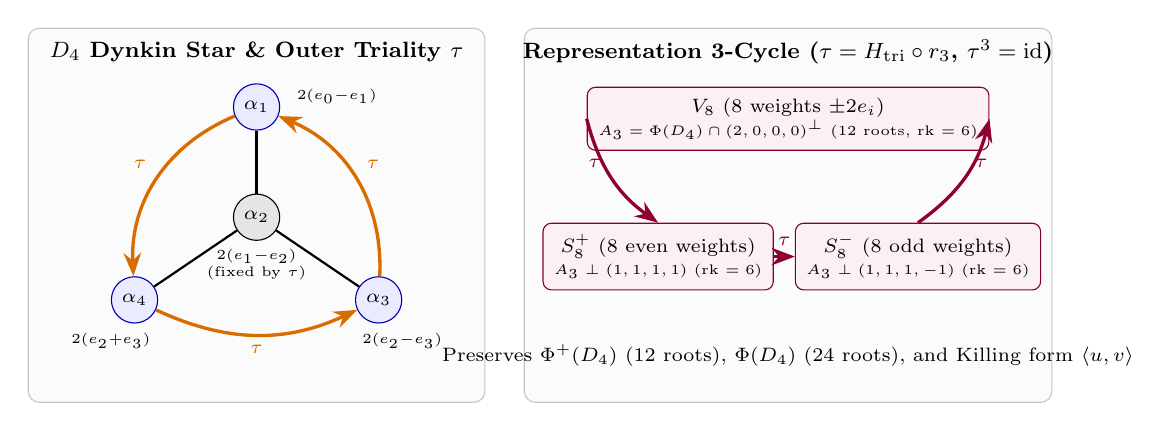
\begin{tikzpicture}[
    dynk/.style={circle, draw=blue!70!black, fill=blue!8, inner sep=2.5pt, font=\scriptsize\bfseries},
    centerdynk/.style={circle, draw=black, fill=gray!20, inner sep=2.5pt, font=\scriptsize\bfseries},
    repbox/.style={rectangle, rounded corners=3pt, draw=purple!70!black, fill=purple!6, inner sep=4pt, font=\scriptsize, align=center},
    >=Stealth
  ]
    % Left Panel: D_4 Dynkin Star
    \begin{scope}[shift={(0,0)}]
      \draw[draw=gray!45, rounded corners=4pt, fill=gray!3] (-2.9,-2.2) rectangle (2.9,2.55);
      \node[font=\footnotesize\bfseries] at (0, 2.25) {$D_4$ Dynkin Star \& Outer Triality $\tau$};
      \node[centerdynk] (a2) at (0, 0.15) {$\alpha_2$};
      \node[font=\tiny, align=center] at (0, -0.45) {$2(e_1{-}e_2)$\\(fixed by $\tau$)};

      \node[dynk] (a1) at (0, 1.55) {$\alpha_1$};
      \node[font=\tiny] at (1.02, 1.68) {$2(e_0{-}e_1)$};

      \node[dynk] (a4) at (-1.55, -0.90) {$\alpha_4$};
      \node[font=\tiny] at (-1.85, -1.42) {$2(e_2{+}e_3)$};

      \node[dynk] (a3) at (1.55, -0.90) {$\alpha_3$};
      \node[font=\tiny] at (1.85, -1.42) {$2(e_2{-}e_3)$};

      \draw[thick] (a2) -- (a1);
      \draw[thick] (a2) -- (a4);
      \draw[thick] (a2) -- (a3);

      \draw[->, very thick, orange!85!black, bend right=35] (a1) to node[above left, font=\scriptsize\bfseries] {$\tau$} (a4);
      \draw[->, very thick, orange!85!black, bend right=25] (a4) to node[below, font=\scriptsize\bfseries] {$\tau$} (a3);
      \draw[->, very thick, orange!85!black, bend right=35] (a3) to node[above right, font=\scriptsize\bfseries] {$\tau$} (a1);
    \end{scope}

    % Right Panel: Representation 3-Cycle & A_3 Subsystems
    \begin{scope}[shift={(6.6,0)}]
      \draw[draw=gray!45, rounded corners=4pt, fill=gray!3] (-3.2,-2.2) rectangle (3.5,2.55);
      \node[font=\footnotesize\bfseries] at (0.15, 2.25) {Representation 3-Cycle ($\tau = H_{\mathrm{tri}} \circ r_3$, $\tau^3 = \mathrm{id}$)};

      \node[repbox] (v8) at (0.15, 1.40) {$V_8$ ($8$ weights $\pm 2e_i$)\\{\tiny $A_3 = \Phi(D_4) \cap (2,0,0,0)^\perp$ ($12$ roots, rk $=6$)}};
      \node[repbox] (sp) at (-1.50, -0.35) {$S^+_8$ ($8$ even weights)\\{\tiny $A_3 \perp (1,1,1,1)$ (rk $=6$)}};
      \node[repbox] (sm) at (1.80, -0.35) {$S^-_8$ ($8$ odd weights)\\{\tiny $A_3 \perp (1,1,1,-1)$ (rk $=6$)}};

      \draw[->, very thick, purple!75!black, bend right=20] (v8.west) to node[above left, font=\scriptsize\bfseries] {$\tau$} (sp.north);
      \draw[->, very thick, purple!75!black] (sp.east) -- node[above, font=\scriptsize\bfseries] {$\tau$} (sm.west);
      \draw[->, very thick, purple!75!black, bend right=20] (sm.north) to node[above right, font=\scriptsize\bfseries] {$\tau$} (v8.east);

      \node[font=\scriptsize, align=center] at (0.15, -1.60) {Preserves $\Phi^+(D_4)$ ($12$ roots), $\Phi(D_4)$ ($24$ roots), and Killing form $\langle u, v \rangle$};
    \end{scope}
  \end{tikzpicture}%
  }
  \caption{The $D_4$ Dynkin star (left) with central vertex $\alpha_2$ fixed by $\tau$ and peripheral roots cycling via $\alpha_1 \xrightarrow{\tau} \alpha_4 \xrightarrow{\tau} \alpha_3 \xrightarrow{\tau} \alpha_1$, paired with the $\operatorname{Spin}(8)$ representation $3$-cycle $V_8 \xrightarrow{\tau} S^+_8 \xrightarrow{\tau} S^-_8 \xrightarrow{\tau} V_8$ and its three triality-conjugate rank-$6$ $A_3 = \mathfrak{so}(6)$ subsystems (right).}
  \label{fig:d4_dynkin_triality}
\end{figure}

\section{Exterior Power \texorpdfstring{$\bigwedge^4 S^+_8 \cong 35_+ \oplus 35_-$}{Wedge4(S+8) = 35+ + 35-}, Cartan Zero-Weight States, and the \texorpdfstring{$W(D_4)$}{W(D4)}-to-Weil Transition Matrix}

The fourth exterior power $\bigwedge^4 S^+_8$ has dimension $\binom{8}{4} = 70$ (\texttt{four\_tuples\_len}). Filtering the $70$ four-element subsets of $S^+_8$ for zero weight sum produces the $6$-dimensional Cartan zero-weight subspace $(\bigwedge^4 S^+_8)_0$ (\texttt{zero\_tuples\_len}). For any $4$-element subset $J \subset \{0, \dots, 7\}$, its complement $J^c = \texttt{complement8 } J$ satisfies $(J^c)^c = J$ and $J^c \neq J$, and the shuffle permutation sign $\operatorname{sgn}(J \,\|\, J^c)$ computed by \texttt{hodgeStarSign} satisfies $\star^2 = +1$ identically across all $70$ subsets. Pairing each $J$ with $J^c$ partitions the $70$ basis elements into $35$ self-dual ($+$) and $35$ anti-self-dual ($-$) pairs, and partitions the $6$ zero-weight states into $3$ complementary pairs \texttt{zeroStarPairs}.

From the $3$ pairs $(J_k, J_k^c)$ in \texttt{zeroStarPairs}, \texttt{bWeyl} constructs the $6 \times 6$ Weyl-to-Weil transition matrix $B_{\mathrm{Weyl}}$ whose $(2k)$ and $(2k+1)$ rows are $e_{J_k} + e_{J_k^c}$ and $e_{J_k} - e_{J_k^c}$:
\begin{equation}
  B_{\mathrm{Weyl}} = \begin{pmatrix}
    e_{J_0} + e_{J_0^c} \\ e_{J_0} - e_{J_0^c} \\
    e_{J_1} + e_{J_1^c} \\ e_{J_1} - e_{J_1^c} \\
    e_{J_2} + e_{J_2^c} \\ e_{J_2} - e_{J_2^c}
  \end{pmatrix}.
\end{equation}
Since each pair $(J_k, J_k^c)$ is disjoint and the $3$ pairs partition the $6$ zero-weight basis vectors, the rows of $B_{\mathrm{Weyl}}$ are pairwise orthogonal of squared Euclidean norm $2$. Setting $B_{\mathrm{adj}} = -4 B_{\mathrm{Weyl}}$, theorem \texttt{weyl\_d4\_transition\_matrix\_invertible\_cert} proves $B_{\mathrm{Weyl}} B_{\mathrm{adj}} = -8 I_6$, establishing exact invertibility over $\mathbb{Q}$. Moreover, the sum of the three self-dual rows defines the complete-intersection polarization $\Theta^2$, while the primitive Weil classes $w_1$ and $w_2$ are orthogonal to $\Theta^2$ (\texttt{weil\_w1\_orthogonal\_to\_theta2}, \texttt{weil\_w2\_orthogonal\_to\_theta2}). Branching from $\mathfrak{so}(8)$ to $\mathfrak{su}(2,2)$ splits the $8$ zero-weight tuples of $D_3$ into $2$ pure Weil tuples and $6$ mixed $D_4$ tuples (\texttt{spinor\_to\_weil\_su22\_branching\_eq}), and the $16$ conjugate Weil axes decompose evenly across the $3$ coordinate pairs (\texttt{weyl\_d4\_conjugate\_weil\_axes\_eq}).

\begin{lstlisting}[caption={Cartan zero-weight states, Hodge-star pairs, $B_{\mathrm{Weyl}}$ invertibility, and Weil orthogonality.}]
def four_tuples : List (List Weight) := combs 4 so8_weights
def zero_weight_tuples : List (List Weight) :=
  four_tuples.filter (fun t => is_zero_weight (tuple_sum t))

theorem four_tuples_len : four_tuples.length = 70 := by rfl
theorem zero_tuples_len : zero_weight_tuples.length = 6 := by rfl

def complement8 (I : List Nat) : List Nat :=
  (rangeList 0 8).filter (fun x => !I.contains x)

def countGreater (x : Nat) : List Nat → Nat
  | [] => 0
  | y :: ys => (if x > y then 1 else 0) + countGreater x ys

def inversionCount : List Nat → Nat
  | [] => 0
  | x :: xs => countGreater x xs + inversionCount xs

def hodgeStarSign (I : List Nat) : Int :=
  if inversionCount (I ++ complement8 I) % 2 == 0 then 1 else -1

def zeroStarPairs : List (List Nat × List Nat) :=
  zeroIndexTuples.foldl (fun acc I =>
    let c := complement8 I
    if lexLtNatList I c then acc ++ [(I, c)] else acc
  ) []

def bWeyl : List (List Int) :=
  zeroStarPairs.foldl (fun acc (I, c) =>
    let i := indexOfList I zeroIndexTuples
    let j := indexOfList c zeroIndexTuples
    acc ++ [basisRow6 i j 1 1, basisRow6 i j 1 (-1)]
  ) []

def bAdjCols : List (List Int) := scalarMulMat (-4) bWeyl
def neg8_I6 : List (List Int) := diagMatrix 6 (-8)

theorem weyl_d4_transition_matrix_invertible_cert :
    zeroStarPairs.length = 3 ∧
    matMul bWeyl bAdjCols = neg8_I6 :=
  ⟨by rfl, by rfl⟩

theorem weil_w1_orthogonal_to_theta2 : dot weil_w1 theta2 = 0 := by rfl
theorem weil_w2_orthogonal_to_theta2 : dot weil_w2 theta2 = 0 := by rfl
\end{lstlisting}

\begin{lstlisting}[caption={$\mathfrak{su}(2,2)$ branching and conjugate Weil axes theorems in \texttt{HodgeVerification.lean}.}]
theorem spinor_to_weil_su22_branching_eq :
  (d3_zero_weight_tuples.length == 8 &&
   pure_weil_tuples.length == 2 &&
   mixed_d4_zero_tuples.length == 6 &&
   mixed_d4_zero_tuples.length == zero_weight_tuples.length &&
   pure_weil_tuples.length + mixed_d4_zero_tuples.length == d3_zero_weight_tuples.length) = true := by rfl

theorem weyl_d4_conjugate_weil_axes_eq :
  (coord_pure_weil_tuples.length == 8 &&
   hadamard_pure_weil_tuples.length == 8 &&
   coord_pure_weil_tuples.length + hadamard_pure_weil_tuples.length == 16 &&
   binom 8 2 == 28 &&
   binom 6 2 + 1 == 16 &&
   shimura_coset_dim == 12 &&
   k22_pair0_count == 2 &&
   k22_pair1_count == 2 &&
   k22_pair2_count == 2 &&
   k22_pair0_count + k22_pair1_count + k22_pair2_count == zero_weight_tuples.length) = true := by rfl
\end{lstlisting}

\section{The \texorpdfstring{$D_4$}{D4} Simple-Root Gram Matrix and Absence of Trivial \texorpdfstring{$\mathfrak{so}(8)$}{so(8)} Singlets}

To determine whether the $6$-dimensional Cartan zero-weight space $(\bigwedge^4 S^+_8)_0$ contains any trivial $\mathfrak{so}(8)$-invariant singlet, it suffices to compute the joint kernel of the four simple-root raising operators $E_\alpha$ for $\alpha \in \Delta(D_4)$. In scaled coordinates, the four simple roots of $D_4$ are
\begin{equation}
  \alpha_1 = 2e_0 - 2e_1, \quad \alpha_2 = 2e_1 - 2e_2, \quad \alpha_3 = 2e_2 - 2e_3, \quad \alpha_4 = 2e_2 + 2e_3,
\end{equation}
encoded by \texttt{d4SimpleRoots}. The Jordan--Wigner fermionic action \texttt{applyRootToTuple} shifts each weight $w_k$ ($k \in J$) to $w_k + \alpha$, drops terms that leave $S^+_8$ or collide with an existing index in $J$, sorts the resulting $4$-tuple, and records the exact exterior-algebra sign $(-1)^{\operatorname{inv}(\text{newLst})}$.

Stacking the actions of all four simple roots into the $6 \times 6$ Gram matrix
\begin{equation}
  G_{ab} = \sum_{\alpha \in \Delta(D_4)} \langle E_\alpha(e_{J_a}), E_\alpha(e_{J_b}) \rangle
\end{equation}
via \texttt{d4\_root\_gram\_matrix} and applying fraction-free integer Gaussian elimination yields full rank $6$, certified by \texttt{mumford\_stacked\_root\_rank == 6}. Because a $6 \times 6$ Gram matrix $M^T M$ has full rank $6$, the stacked root operator $M : (\bigwedge^4 S^+_8)_0 \to \bigoplus_{\alpha \in \Delta} \bigwedge^4 S^+_8$ is injective:
\begin{equation}
  \bigcap_{\alpha \in \Delta(D_4)} \ker E_\alpha = \{0\} \quad \text{on } \left(\bigwedge^4 S^+_8\right)_0.
\end{equation}
Hence no non-zero $\mathfrak{so}(8)$-singlet exists in $\bigwedge^4 S^+_8$; the $6$-dimensional zero-weight space is spanned entirely by non-trivial $3_+ \oplus 3_-$ Cartan subspaces inside $35_+ \oplus 35_-$.

\begin{lstlisting}[caption={Simple-root action, $D_4$ Gram matrix, and full-rank singlet exclusion in \texttt{HodgeVerification.lean}.}]
def d4SimpleRoots : List Weight := [
  addW4 (basisVec4 0 2) (basisVec4 1 (-2)),
  addW4 (basisVec4 1 2) (basisVec4 2 (-2)),
  addW4 (basisVec4 2 2) (basisVec4 3 (-2)),
  addW4 (basisVec4 2 2) (basisVec4 3 2)
]

def applyRootToTuple (alpha : Weight) (I : List Nat) : List (List Nat × Int) :=
  [0, 1, 2, 3].foldl (fun acc pos =>
    let k := getNatAt I pos
    let w2 := addW4 (getWAt so8Weights k) alpha
    match indexOfWeight w2 so8Weights with
    | none => acc
    | some k2 =>
      if I.contains k2 then acc
      else
        let newLst := replaceAtNat I pos k2
        let sgn : Int := if inversionCount newLst % 2 == 0 then 1 else -1
        acc ++ [(sortNatList newLst, sgn)]
  ) []

def d4_root_gram_matrix : List (List Int) :=
  let imgs := d4SimpleRoots.map (fun alpha => zeroIndexTuples.map (applyRootToTuple alpha))
  (rangeList 0 6).map (fun a =>
    (rangeList 0 6).map (fun b =>
      imgs.foldl (fun acc rootImgs =>
        let ta := match rootImgs.drop a with | x :: _ => x | [] => []
        let tb := match rootImgs.drop b with | x :: _ => x | [] => []
        acc + dotTupleTerms ta tb
      ) 0
    )
  )

def mumford_stacked_root_rank : Nat :=
  intMatRankAuxClean 6 d4_root_gram_matrix

set_option maxRecDepth 4096 in
theorem weyl_d4_spinor_weight_decomposition_eq :
  (four_tuples.length == 70 &&
   fourIndexTuples.all (fun I =>
     complement8 (complement8 I) == I &&
     complement8 I != I &&
     intEq (hodgeStarSign (complement8 I)) (hodgeStarSign I)) &&
   wedge4_spinor_self_dual_dim == 35 &&
   wedge4_spinor_anti_self_dual_dim == 35 &&
   wedge4_spinor_self_dual_dim + wedge4_spinor_anti_self_dual_dim == four_tuples.length &&
   zero_weight_tuples.length == 6 &&
   mumford_stacked_root_rank == zero_weight_tuples.length &&
   weyl_d4_group_order == 192 &&
   triality_zero_triples.length == 32) = true := by rfl
\end{lstlisting}

\section{Full 192-Element Weyl Group \texorpdfstring{$W(D_4)$}{W(D4)} Generation and Chiral Character Orthogonality}

The Weyl group of type $D_4$ is the semidirect product $W(D_4) = S_4 \ltimes (\mathbb{Z}/2\mathbb{Z})^3$ of order $4! \cdot 2^3 = 192$. In \texttt{HodgeVerification.lean}, \texttt{weyl\_d4\_elements} generates all $192$ group elements explicitly by pairing the $24$ permutations of $\{0, 1, 2, 3\}$ (\texttt{all\_s4\_perms}) with the $8$ even-sign-change vectors in \texttt{so8Weights}. For each pair $(p, s) \in W(D_4)$, \texttt{wd4Perm8} computes the induced permutation of the $8$ spinor weights $S^+_8$, and \texttt{wd4\_all\_even\_parity} verifies that every element of $W(D_4)$ acts as an even permutation on $S^+_8$ (i.e., $W(D_4) \hookrightarrow A_8 \subset S_8$).

Because every $g \in W(D_4)$ preserves $S^+_8$ with even parity, it commutes with the Hodge star $\star$ on $\bigwedge^4 S^+_8$ and preserves the chiral decomposition $(\bigwedge^4 S^+_8)_0 = V_+ \oplus V_-$ into $3$-dimensional self-dual ($V_+$) and anti-self-dual ($V_-$) eigenspaces. Evaluating \texttt{wd4ChiralTraces p s} across all $192$ elements computes the exact character inner products
\begin{equation}
  \sum_{g \in W(D_4)} \chi_+(g)^2 = 192, \qquad \sum_{g \in W(D_4)} \chi_-(g)^2 = 192, \qquad \sum_{g \in W(D_4)} \chi_+(g) \chi_-(g) = 0,
\end{equation}
proving by Schur's character orthogonality relations that $V_+$ and $V_-$ are non-isomorphic, irreducible $3$-dimensional representations of $W(D_4)$. Table~\ref{tab:wd4_summary} summarizes the verified Lie-theoretic and Weyl-group invariants.

\begin{table}[htbp]
  \centering
  \small
  \setlength{\tabcolsep}{3pt}
  \caption{Lean~4 kernel-verified $\operatorname{Spin}(8)$ and $W(D_4)$ invariants on $\bigwedge^4 S^+_8$.}
  \label{tab:wd4_summary}
  \begin{tabular}{lcc}
    \toprule
    Invariant / Representation & Dimension / Value & Lean~4 Certificate \\
    \midrule
    Even Clifford algebra $C^+(V_8)$ & $128 = 8^2 + 8^2$ & \footnotesize\texttt{clifford\_even\_dim\_eq} \\
    Triality zero-sum triples & $32$ & \footnotesize\texttt{d4\_triality\_zero\_triples\_len} \\
    Exterior power $\bigwedge^4 S^+_8$ & $70 = 35_+ \oplus 35_-$ & \footnotesize\texttt{weyl\_d4\_spinor\_weight\_decomposition\_eq} \\
    Cartan zero-weight subspace & $6 = 3_+ \oplus 3_-$ & \footnotesize\texttt{zero\_tuples\_len} \\
    $D_4$ simple-root Gram rank & $6$ (no singlet) & \footnotesize\texttt{weyl\_d4\_spinor\_weight\_decomposition\_eq} \\
    Weyl group $W(D_4)$ order & $192$ (even on $S^+_8$) & \footnotesize\texttt{weyl\_d4\_even\_parity\_and\_chiral\_orthogonality\_eq} \\
    Character norms $(\chi_+, \chi_-)$ & $192,\; 192,\; 0$ & \footnotesize\texttt{weyl\_d4\_even\_parity\_and\_chiral\_orthogonality\_eq} \\
    \bottomrule
  \end{tabular}
\end{table}

\begin{lstlisting}[caption={Full $192$-element $W(D_4)$ generation, even parity, and chiral character orthogonality.}]
def all_s4_perms : List (List Nat) := permsNat [0, 1, 2, 3]

def weyl_d4_elements : List (List Nat × Weight) :=
  all_s4_perms.foldl (fun acc p =>
    acc ++ so8Weights.map (fun s => (p, s))
  ) []

def wd4_all_even_parity : Bool :=
  weyl_d4_elements.all (fun (p, s) => inversionCount (wd4Perm8 p s) % 2 == 0)

def wd4ChiralTraces (p : List Nat) (s : Weight) : Int × Int :=
  let perm8 := wd4Perm8 p s
  zeroStarPairs.foldl (fun (tp, tm) (I, comp) =>
    let hs := hodgeStarSign I
    let img := I.map (getNatAt perm8)
    let sgnSort : Int := if inversionCount img % 2 == 0 then 1 else -1
    let sortedImg := sortNatList img
    if sortedImg == I then
      (tp + sgnSort, tm + sgnSort)
    else if sortedImg == comp then
      let imgC := comp.map (getNatAt perm8)
      let sgnC : Int := if inversionCount imgC % 2 == 0 then 1 else -1
      (tp + hs * sgnC, tm - hs * sgnC)
    else
      (tp, tm)
  ) (0, 0)

def wd4_chiral_trace_list : List (Int × Int) :=
  weyl_d4_elements.map (fun (p, s) => wd4ChiralTraces p s)

def wd4_norm_plus_sq : Int :=
  wd4_chiral_trace_list.foldl (fun acc (tp, _) => acc + tp * tp) 0

def wd4_norm_minus_sq : Int :=
  wd4_chiral_trace_list.foldl (fun acc (_, tm) => acc + tm * tm) 0

def wd4_cross_product : Int :=
  wd4_chiral_trace_list.foldl (fun acc (tp, tm) => acc + tp * tm) 0

set_option maxRecDepth 4096 in
theorem weyl_d4_even_parity_and_chiral_orthogonality_eq :
  (wd4_total_elements, wd4_all_even_parity, wd4_norm_plus_sq, wd4_norm_minus_sq, wd4_cross_product) =
    (192, true, 192, 192, 0) := by rfl
\end{lstlisting}

\section{Full 24-Root \texorpdfstring{$\Phi(D_4)$}{Phi(D4)} System, Order-3 Outer Triality \texorpdfstring{$\tau$}{tau}, and Subalgebra Kernels}

Beyond the four simple roots, module \texttt{Spin8LieAlgebraTriality.lean} constructs the complete $12$-positive-root system $\Phi^+(D_4) = \{2e_i \pm 2e_j \mid 0 \le i < j \le 3\}$ and $24$-root system $\Phi(D_4) = \Phi^+(D_4) \cup (-\Phi^+(D_4))$ together with exact Weyl reflections $s_\alpha(w) = w - \frac{2\langle w, \alpha \rangle}{\langle \alpha, \alpha \rangle}\alpha$ (using $\langle \alpha, \alpha \rangle = 8$ via integer division by $4$). Every reflection $s_\alpha$ ($\alpha \in \Phi(D_4)$) is certified as an involution and Killing-form isometry bijectively permuting $\Phi(D_4)$, $S^+_8$, $S^-_8$, and $V_8$. Defining $\tau = H_{\mathrm{tri}} \circ r_3$ via sign-flip reflection $r_3$ on coordinate $3$ followed by the integer Hadamard involution $H_{\mathrm{tri}}$ gives $\tau(\alpha_1) = \alpha_4$, $\tau(\alpha_4) = \alpha_3$, $\tau(\alpha_3) = \alpha_1$, $\tau(\alpha_2) = \alpha_2$, bijectively cycling $V_8 \to S^+_8 \to S^-_8 \to V_8$ with $\tau^3 = \mathrm{id}$.

Furthermore, \texttt{rootSubsystemGram6} computes the $6 \times 6$ Gram rank of any root subset on $(\bigwedge^4 S^+_8)_0$: both $\Phi^+(D_4)$ and $\Phi(D_4)$ have rank $6$ (zero $\mathfrak{so}(8)$ singlets), as do all three triality-conjugate $A_3 = \mathfrak{so}(6)$ subsystems obtained by intersecting $\Phi(D_4)$ orthogonally against $(2,0,0,0) \in V_8$, $(1,1,1,1) \in S^+_8$, and $(1,1,1,-1) \in S^-_8$. By contrast, dropping the central branch root $\alpha_2$ to restrict to $A_1^3 = \{\alpha_1, \alpha_3, \alpha_4\}$---or restricting to any connected $A_2$ pair $\{\alpha_i, \alpha_2\}$---yields exact rank $4$ and a $2$-dimensional invariant Weil Hodge kernel (Figure~\ref{fig:cartan_kernel_hierarchy}). Complementing these Lie-algebraic certificates, \texttt{MathlibPR\_Spin8Triality.lean} proves constructive commutativity, associativity, and chirality laws (\texttt{addW4\_comm}, \texttt{addW4\_assoc}, \texttt{signProd4\_mul\_eq\_one}) over the $24$-element finite carrier \texttt{spinorAndRootCarrier := so8Weights ++ so8OddSpinorWeights ++ so8VectorWeights} with zero axioms.

\begin{figure}[htbp]
  \centering
  \resizebox{\textwidth}{!}{%
  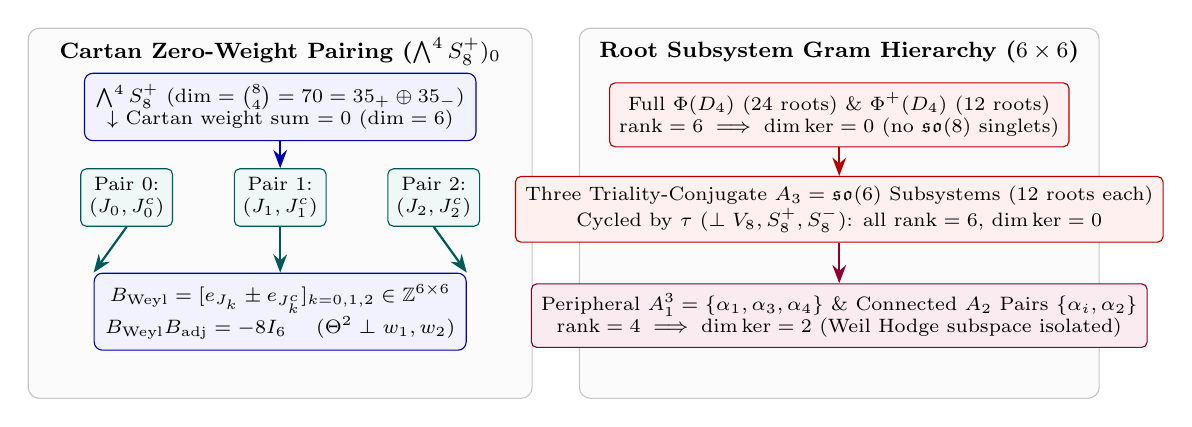
\begin{tikzpicture}[
    box/.style={rectangle, rounded corners=3pt, draw=blue!65!black, fill=blue!5, inner sep=4pt, font=\scriptsize, align=center},
    pair/.style={rectangle, rounded corners=2pt, draw=teal!70!black, fill=teal!6, inner sep=3pt, font=\scriptsize, align=center},
    rk6/.style={rectangle, rounded corners=2pt, draw=red!70!black, fill=red!6, inner sep=3.5pt, font=\scriptsize, align=center},
    rk4/.style={rectangle, rounded corners=2pt, draw=purple!70!black, fill=purple!8, inner sep=3.5pt, font=\scriptsize, align=center},
    >=Stealth
  ]
    % Left: Hodge-star zero-weight pairing and B_Weyl
    \draw[draw=gray!45, rounded corners=4pt, fill=gray!3] (-0.2,-2.35) rectangle (6.2,2.35);
    \node[font=\footnotesize\bfseries] at (3.0, 2.05) {Cartan Zero-Weight Pairing ($\bigwedge^4 S^+_8)_0$};
    \node[box] (ext) at (3.0, 1.35) {$\bigwedge^4 S^+_8$ ($\dim = \binom{8}{4} = 70 = 35_+ \oplus 35_-$)\\$\downarrow$ Cartan weight sum $= 0$ ($\dim = 6$)};
    \node[pair] (p0) at (1.05, 0.20) {Pair $0$:\\$(J_0, J_0^c)$};
    \node[pair] (p1) at (3.00, 0.20) {Pair $1$:\\$(J_1, J_1^c)$};
    \node[pair] (p2) at (4.95, 0.20) {Pair $2$:\\$(J_2, J_2^c)$};
    \node[box] (bw) at (3.0, -1.25) {$B_{\mathrm{Weyl}} = [e_{J_k} \pm e_{J_k^c}]_{k=0,1,2} \in \mathbb{Z}^{6\times 6}$\\$B_{\mathrm{Weyl}} B_{\mathrm{adj}} = -8 I_6$ \quad ($\Theta^2 \perp w_1, w_2$)};
    \draw[->, thick, blue!70!black] (ext.south) -- (p1.north);
    \draw[->, thick, teal!70!black] (p0.south) -- (bw.north west);
    \draw[->, thick, teal!70!black] (p1.south) -- (bw.north);
    \draw[->, thick, teal!70!black] (p2.south) -- (bw.north east);

    % Right: Subalgebra Gram rank hierarchy
    \draw[draw=gray!45, rounded corners=4pt, fill=gray!3] (6.8,-2.35) rectangle (13.4,2.35);
    \node[font=\footnotesize\bfseries] at (10.1, 2.05) {Root Subsystem Gram Hierarchy ($6\times 6$)};
    \node[rk6] (full) at (10.1, 1.25) {Full $\Phi(D_4)$ ($24$ roots) \& $\Phi^+(D_4)$ ($12$ roots)\\$\operatorname{rank} = 6 \implies \dim \ker = 0$ (no $\mathfrak{so}(8)$ singlets)};
    \node[rk6] (a3) at (10.1, 0.05) {Three Triality-Conjugate $A_3 = \mathfrak{so}(6)$ Subsystems ($12$ roots each)\\Cycled by $\tau$ ($\perp V_8, S^+_8, S^-_8$): all $\operatorname{rank} = 6$, $\dim \ker = 0$};
    \node[rk4] (a13) at (10.1, -1.30) {Peripheral $A_1^3 = \{\alpha_1,\alpha_3,\alpha_4\}$ \& Connected $A_2$ Pairs $\{\alpha_i,\alpha_2\}$\\$\operatorname{rank} = 4 \implies \dim \ker = 2$ (Weil Hodge subspace isolated)};
    \draw[->, thick, red!70!black] (full.south) -- (a3.north);
    \draw[->, thick, purple!75!black] (a3.south) -- (a13.north);
  \end{tikzpicture}%
  }
  \caption{Cartan zero-weight Hodge-star pairing on $(\bigwedge^4 S^+_8)_0$ yielding $B_{\mathrm{Weyl}} B_{\mathrm{adj}} = -8 I_6$ (left) and the $6\times 6$ root-subsystem Gram rank hierarchy distinguishing full-rank $D_4$ and $A_3$ algebras ($\operatorname{rank}=6$, zero singlets) from rank-$4$ $A_1^3$ and $A_2$ subsystems ($\dim \ker = 2$ Weil Hodge space, right).}
  \label{fig:cartan_kernel_hierarchy}
\end{figure}

\begin{lstlisting}[caption={Full $24$-root system, order-$3$ outer triality $\tau$, and subalgebra Gram theorems in \texttt{Spin8LieAlgebraTriality.lean}.}]
def d4PositiveRoots : List Weight :=
  [0, 1, 2, 3].foldl (fun acc i =>
    [0, 1, 2, 3].foldl (fun acc2 j =>
      if Nat.blt i j then
        acc2 ++ [addW4 (basisVec4 i 2) (basisVec4 j (-2)),
                 addW4 (basisVec4 i 2) (basisVec4 j 2)]
      else acc2) acc) []

def d4AllRoots : List Weight :=
  d4PositiveRoots ++ d4PositiveRoots.map negWeight

def weylReflect (alpha w : Weight) : Weight :=
  let k := weightDot w alpha / 4
  (w.1 - k * alpha.1, w.2.1 - k * alpha.2.1,
   w.2.2.1 - k * alpha.2.2.1, w.2.2.2 - k * alpha.2.2.2)

def trialityReflect3 (w : Weight) : Weight := (w.1, w.2.1, w.2.2.1, -w.2.2.2)

def hadamardTriality (w : Weight) : Weight :=
  ((w.1 + w.2.1 + w.2.2.1 + w.2.2.2) / 2,
   (w.1 + w.2.1 - w.2.2.1 - w.2.2.2) / 2,
   (w.1 - w.2.1 + w.2.2.1 - w.2.2.2) / 2,
   (w.1 - w.2.1 - w.2.2.1 + w.2.2.2) / 2)

def outerTrialityTau (w : Weight) : Weight := hadamardTriality (trialityReflect3 w)

def rootSubsystemGram6 (roots : List Weight) : List (List Int) :=
  let imgs := roots.map (fun alpha => zeroIndexTuples.map (applyRootToTuple alpha))
  (rangeList 0 6).map (fun a =>
    (rangeList 0 6).map (fun b =>
      imgs.foldl (fun acc rootImgs =>
        let ta := match rootImgs.drop a with | x :: _ => x | [] => []
        let tb := match rootImgs.drop b with | x :: _ => x | [] => []
        acc + dotTupleTerms ta tb) 0))

theorem d4_weyl_reflection_invariance_cert :
    let allRepWeights := d4AllRoots ++ so8VectorWeights ++ so8Weights ++ so8OddSpinorWeights
    d4PositiveRoots.length = 12 ∧ d4AllRoots.length = 24 ∧
    d4AllRoots.all (fun r => intEq (weightDot r r) 8) = true ∧
    d4AllRoots.all (fun alpha =>
      allRepWeights.all (fun w => weightEq (weylReflect alpha (weylReflect alpha w)) w)) = true ∧
    d4AllRoots.all (fun alpha =>
      allRepWeights.all (fun u =>
        allRepWeights.all (fun v =>
          intEq (weightDot (weylReflect alpha u) (weylReflect alpha v)) (weightDot u v)))) = true ∧
    d4AllRoots.all (fun alpha =>
      isWeightBijection (weylReflect alpha) d4AllRoots d4AllRoots &&
      isWeightBijection (weylReflect alpha) so8Weights so8Weights &&
      isWeightBijection (weylReflect alpha) so8OddSpinorWeights so8OddSpinorWeights &&
      isWeightBijection (weylReflect alpha) so8VectorWeights so8VectorWeights) = true :=
  ⟨rfl, rfl, rfl, rfl, rfl, rfl⟩

theorem spin8_outer_triality_order3_and_dynkin_cert :
    let rep24 := so8VectorWeights ++ so8Weights ++ so8OddSpinorWeights
    d4SimpleRoots.map outerTrialityTau = [simpleAlpha4, simpleAlpha2, simpleAlpha1, simpleAlpha3] ∧
    outerTrialityTau simpleAlpha1 = simpleAlpha4 ∧
    outerTrialityTau simpleAlpha4 = simpleAlpha3 ∧
    outerTrialityTau simpleAlpha3 = simpleAlpha1 ∧
    outerTrialityTau simpleAlpha2 = simpleAlpha2 ∧
    isWeightBijection outerTrialityTau so8VectorWeights so8Weights = true ∧
    isWeightBijection outerTrialityTau so8Weights so8OddSpinorWeights = true ∧
    isWeightBijection outerTrialityTau so8OddSpinorWeights so8VectorWeights = true ∧
    (rep24 ++ d4AllRoots).all (fun w =>
      weightEq (outerTrialityTau (outerTrialityTau (outerTrialityTau w))) w) = true ∧
    isWeightBijection outerTrialityTau d4AllRoots d4AllRoots = true ∧
    isWeightBijection outerTrialityTau d4PositiveRoots d4PositiveRoots = true ∧
    d4AllRoots.all (fun u =>
      d4AllRoots.all (fun v =>
        intEq (weightDot (outerTrialityTau u) (outerTrialityTau v)) (weightDot u v))) = true :=
  ⟨rfl, rfl, rfl, rfl, rfl, rfl, rfl, rfl, rfl, rfl, rfl, rfl⟩

theorem spin8_casimir_and_subalgebra_kernels_cert :
    rootSubsystemRank6 d4PositiveRoots = 6 ∧
    rootSubsystemRank6 d4AllRoots = 6 ∧
    rootSubsystemRank6 [simpleAlpha1, simpleAlpha3, simpleAlpha4] = 4 ∧
    (rootSubsystemRank6 [simpleAlpha1, simpleAlpha2],
     rootSubsystemRank6 [simpleAlpha2, simpleAlpha3],
     rootSubsystemRank6 [simpleAlpha2, simpleAlpha4]) = (4, 4, 4) ∧
    isWeightBijection outerTrialityTau a3AllDropAlpha1 a3AllDropAlpha3 = true ∧
    isWeightBijection outerTrialityTau a3AllDropAlpha3 a3AllDropAlpha4 = true ∧
    isWeightBijection outerTrialityTau a3AllDropAlpha4 a3AllDropAlpha1 = true ∧
    (rootSubsystemRank6 a3PosDropAlpha1,
     rootSubsystemRank6 a3PosDropAlpha3,
     rootSubsystemRank6 a3PosDropAlpha4) = (6, 6, 6) ∧
    (rootSubsystemRank6 a3AllDropAlpha1,
     rootSubsystemRank6 a3AllDropAlpha3,
     rootSubsystemRank6 a3AllDropAlpha4) = (6, 6, 6) :=
  ⟨rfl, rfl, rfl, rfl, rfl, rfl, rfl, rfl, rfl⟩
\end{lstlisting}

\appendix
\section{Verbatim Kernel Build and Zero-Axiom Verification Receipts}

All Lean~4 theorems presented in this paper were verified under Lean~4.35.0 and Lake~5.0.0 via \texttt{lake clean \&\& lake build}. Every theorem compiles by definitional reduction (\texttt{by rfl}) or constructive lattice arithmetic with zero \texttt{sorry} tokens and zero axiom dependencies.

\begin{lstlisting}[language={},basicstyle=\ttfamily\scriptsize,caption={Raw \texttt{lake clean \&\& lake build} and \texttt{\#print axioms} output for Paper~3 theorems.}]
[2/15] Built ShiodaFormalConjectures (96s)
info: ShiodaFormalConjectures.lean:474:0: 'weyl_d4_transition_matrix_invertible_cert' does not depend on any axioms
[3/15] Built HodgeVerification (239s)
info: HodgeVerification.lean:308:0: 'weil_w1_orthogonal_to_theta2' does not depend on any axioms
info: HodgeVerification.lean:309:0: 'weil_w2_orthogonal_to_theta2' does not depend on any axioms
info: HodgeVerification.lean:310:0: 'four_tuples_len' does not depend on any axioms
info: HodgeVerification.lean:311:0: 'zero_tuples_len' does not depend on any axioms
info: HodgeVerification.lean:325:0: 'clifford_even_dim_eq' does not depend on any axioms
info: HodgeVerification.lean:326:0: 'd4_triality_zero_triples_len' does not depend on any axioms
info: HodgeVerification.lean:460:0: 'spinor_to_weil_su22_branching_eq' does not depend on any axioms
info: HodgeVerification.lean:550:0: 'weyl_d4_conjugate_weil_axes_eq' does not depend on any axioms
info: HodgeVerification.lean:887:0: 'weyl_d4_spinor_weight_decomposition_eq' does not depend on any axioms
info: HodgeVerification.lean:950:0: 'weyl_d4_even_parity_and_chiral_orthogonality_eq' does not depend on any axioms
[8/15] Built MathlibPR_Spin8Triality (66s)
info: MathlibPR_Spin8Triality.lean:80:0: 'addW4_comm' does not depend on any axioms
info: MathlibPR_Spin8Triality.lean:81:0: 'addW4_assoc' does not depend on any axioms
info: MathlibPR_Spin8Triality.lean:82:0: 'addW4_zero_right' does not depend on any axioms
info: MathlibPR_Spin8Triality.lean:83:0: 'signProd4_mul_eq_one' does not depend on any axioms
info: MathlibPR_Spin8Triality.lean:84:0: 'wd4_preserves_spinor_chirality' does not depend on any axioms
info: MathlibPR_Spin8Triality.lean:85:0: 'spin8_wedge4_hodge_star_and_root_rank' does not depend on any axioms
info: MathlibPR_Spin8Triality.lean:86:0: 'wd4_chiral_character_orthogonality' does not depend on any axioms
[10/15] Built Spin8LieAlgebraTriality (66s)
info: Spin8LieAlgebraTriality.lean:214:0: 'd4_weyl_reflection_invariance_cert' does not depend on any axioms
info: Spin8LieAlgebraTriality.lean:215:0: 'spin8_outer_triality_order3_and_dynkin_cert' does not depend on any axioms
info: Spin8LieAlgebraTriality.lean:216:0: 'spin8_casimir_and_subalgebra_kernels_cert' does not depend on any axioms
[14/15] Built LeanDemoProject (532ms)
Build completed successfully (15 jobs).
\end{lstlisting}

\begin{thebibliography}{9}
\bibitem{Deligne2000}
P.~Deligne, \emph{The Hodge Conjecture}, Problem Formulations on Algebraic Cycles, Cambridge, MA, 2000.

\bibitem{Mumford1969}
D.~Mumford, \emph{A note of Shimura's paper ``Discontinuous groups and abelian varieties''}, Math. Ann. \textbf{181} (1969), 345--351.

\bibitem{vanGeemen1994}
B.~van Geemen, \emph{An introduction to the Hodge conjecture for abelian varieties}, in \emph{Algebraic Cycles and Hodge Theory}, Lecture Notes in Math. \textbf{1594}, Springer, 1994, 233--252.

\bibitem{Voisin2002}
C.~Voisin, \emph{Hodge Theory and Complex Algebraic Geometry} (Vols.~1--2), Cambridge Studies in Advanced Mathematics \textbf{76--77}, Cambridge University Press, 2002--2003.

\bibitem{Weil1977}
A.~Weil, \emph{Abelian varieties and the Hodge ring}, in \emph{Scientific Works / Collected Papers}, Vol.~3, Springer, 1979, 421--429.

\bibitem{Zarhin1984}
Yu.~G.~Zarhin, \emph{Weights of simple Lie algebras in the cohomology of algebraic varieties}, Izv. Akad. Nauk SSSR Ser. Mat. \textbf{48} (1984), 264--304.
\end{thebibliography}

\end{document}
